\begin{frame}
\frametitle{Video Selection}
\large{Preconsiderations}

\begin{itemize}
\item Large variety between the reference video files
\item Get \textit{UHD-1} content from public video databases with high quality
\item Sequence: length of 10 seconds (HAS-segment), no cuts, smallest permitted frame rate: 50 fps
\end{itemize}

\end{frame}


\begin{frame}
\frametitle{Video Selection}
\large{Dataset Preparation}

\begin{itemize}
	
\item Main challenge: 
\newline Find periods of video without cuts that are 10 sec or longer
\item Database:
\newline Harmonic \cite{web:harmonic}, Cable Labs \cite{web:cablelabs}, Blender Foundation \cite{web:bbb}.
\item Preselection with a 4k screen:
\newline Get a large variety between the reference video files to evoke different encoding properties

\end{itemize}
\end{frame}


\begin{frame}
\frametitle{Video Selection}

\begin{figure}[hbt!]
	\begin{center}
		%
		
		\subfigure[Air Show]{%
			\label{fig:airshow}
			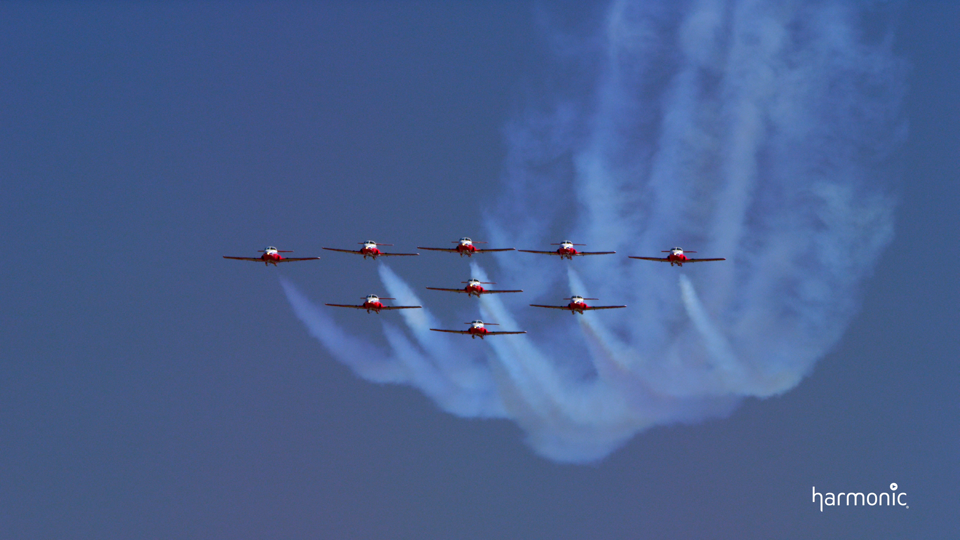
\includegraphics[width=0.3\textwidth]{images/AirShow}
		}%
		\subfigure[Big Buck Bunny]{%
			\label{fig:bbb}
			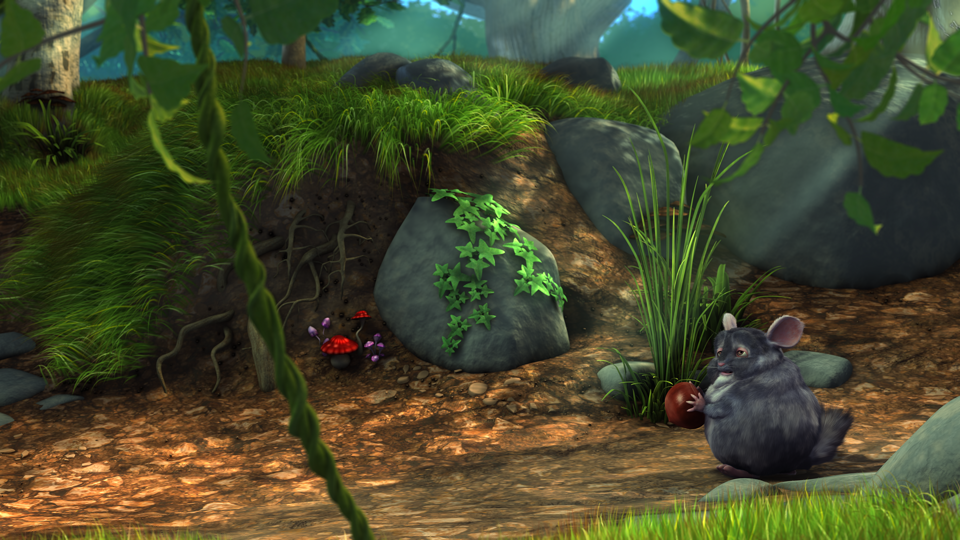
\includegraphics[width=0.3\textwidth]{images/Bbb}
		}
		\subfigure[Fjord]{%
			\label{fig:Fjord}
			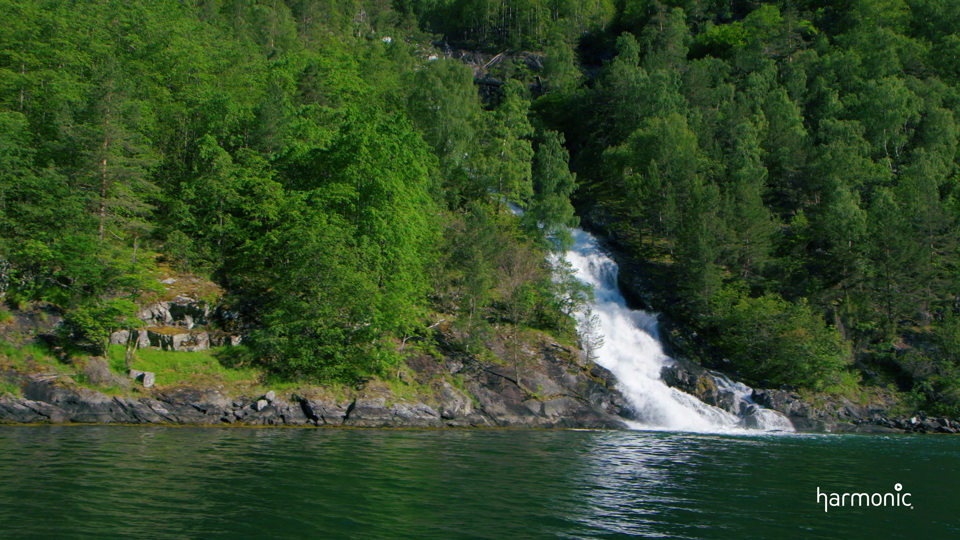
\includegraphics[width=0.3\textwidth]{images/Fjord}
		}\\ %  ------- End of the first row ----------------------%
		\subfigure[Moment of Intensity]{%
			\label{fig:MomentOfIntensity}
			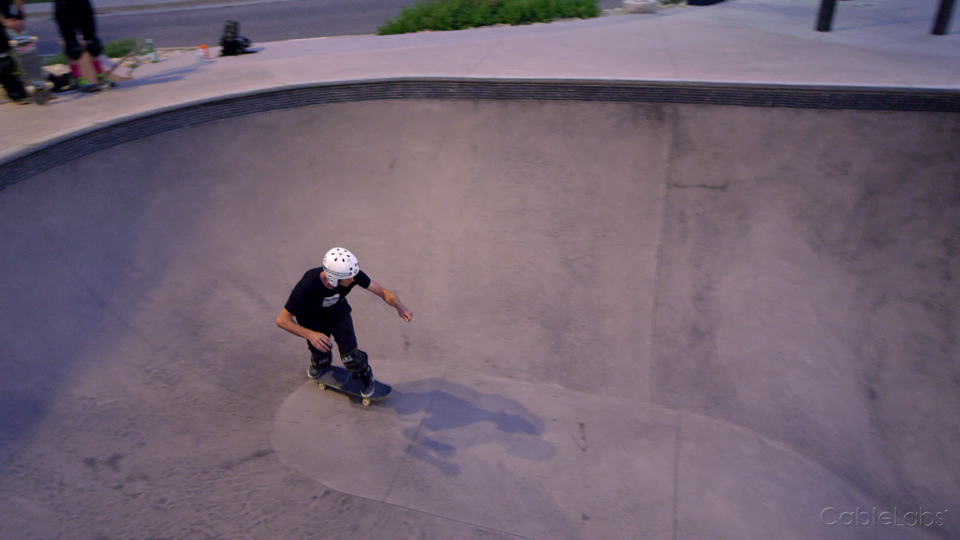
\includegraphics[width=0.3\textwidth]{images/MomentOfIntensity}
		}		
		\subfigure[Snow Monkeys]{%
			\label{fig:SnowMonkeys}
			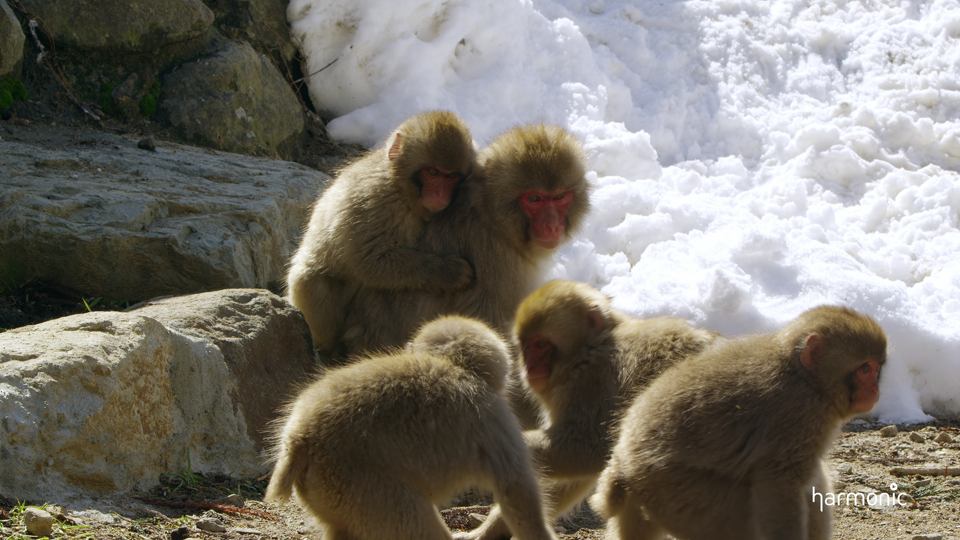
\includegraphics[width=0.3\textwidth]{images/SnowMonkeys}
		}%
		\subfigure[Streets of India]{%
			\label{fig:StreetsOfIndia}
			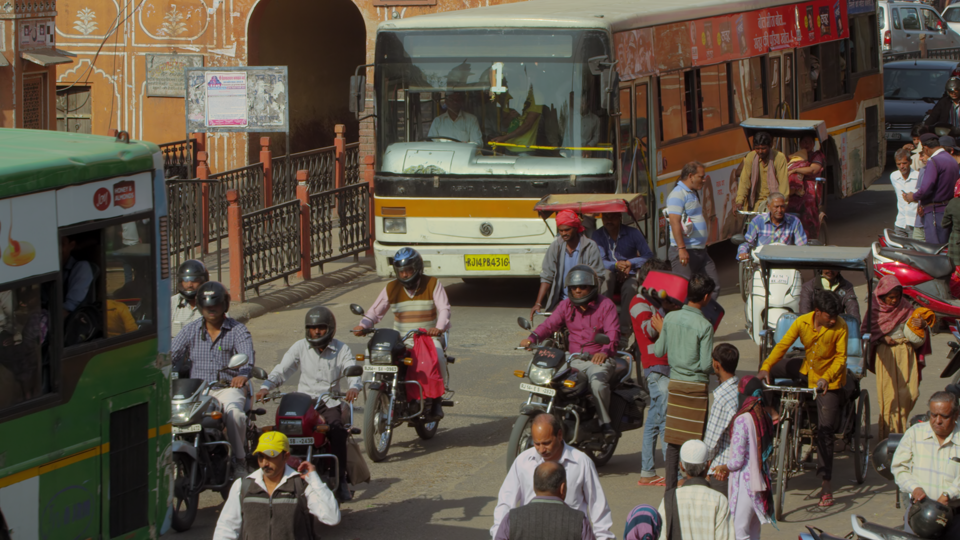
\includegraphics[width=0.3\textwidth]{images/StreetsOfIndia}
		}%
		%
	\end{center}

\end{figure}

Selection of frames contained in the reference videos to show the variety of the content.
\end{frame}


\begin{frame}
\frametitle{Video Selection}

\begin{figure}[hbt!]
	\centering
	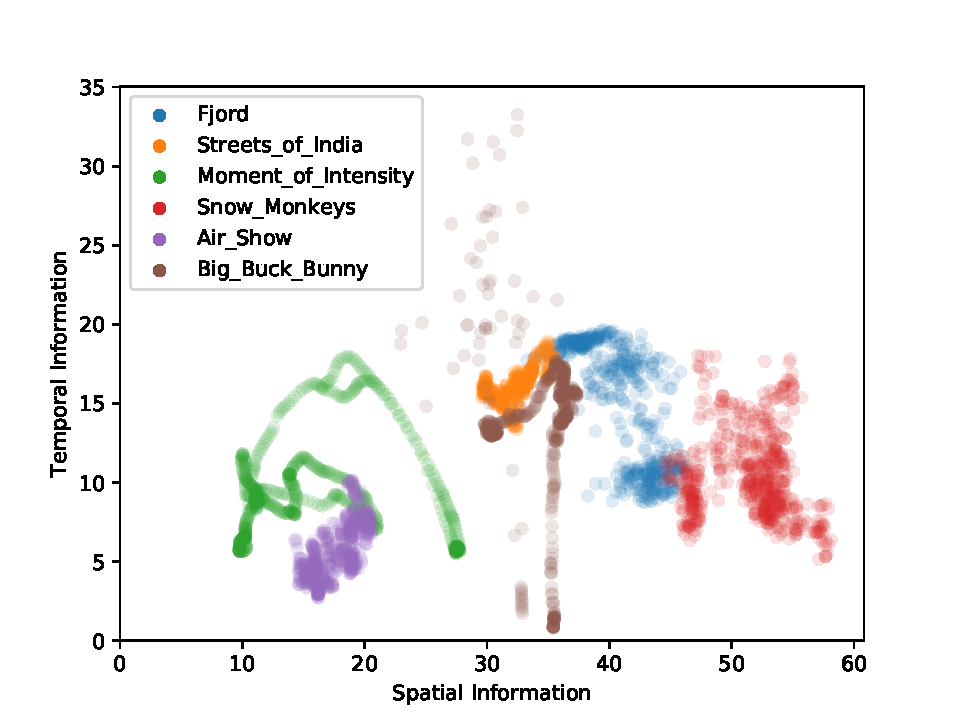
\includegraphics[width=2.9in]{SITI}
\end{figure}

Spatial and temporal information of the reference video files.
\newline Each dot represents one frame.


\end{frame}


